\section{Gestion des tournois}

Cette page permet de gérer tous les tournoi. Pour accéder à cette page, il faut être un membre du staff qui possède les permissions pour gérer les tournois (voir la section Gestion des permissions). \newline

La gestion des tournois comprend, en particulier, la gestion des poules et la gestion des arbres d'élimination de ces tournois.

\begin{figure}[H]
\centering
\includegraphics[scale=0.15]{user_images/staff/GererTournois/001.jpg}
\caption{Gestionnaire des tournois}
\end{figure}

\subsection{Création des poules}

Pour créer les poules d'un tournoi, il faut cliquer sur le bouton à la ligne du tournoi voulu, à la colonne "Générer Poules". Dans l'image ci-dessous, on choisi de cliquer sur le bouton "Générer Poules" du tournoi "Double mixte : Seniors".

\begin{figure}[H]
\centering
\includegraphics[scale=0.15]{user_images/staff/GererTournois/GererPoules/ModifierEtValiderPoules/001.jpg}
\caption{Création des poules, étape 1}
\end{figure}

Sur cette page, on peut personnalisé les poules du tournoi. L'interface est dynamique, et propose de modifier le nombre, la taille des poules, les leaders, terrains, et joueurs des poules. Pour choisir le leader, il suffit de sélectionner un joueur de la poule sur la liste déroulante en haut de la poule correspondante.

\begin{figure}[H]
\centering
\includegraphics[scale=0.15]{user_images/staff/GererTournois/GererPoules/ModifierEtValiderPoules/002.jpg}
\caption{Création des poules, étape 2}
\end{figure}

Pour choisir un terrain de la poule, il suffit de sélectionner le terrain dans la liste déroulante, en dessous de la poule correspondante. Après sélection du terrain, les informations du terrain s'afficheront.

\begin{figure}[H]
\centering
\includegraphics[scale=0.15]{user_images/staff/GererTournois/GererPoules/ModifierEtValiderPoules/003.jpg}
\caption{Création des poules, étape 3}
\end{figure}

Pour modifier la disposition des joueurs dans les poules, il est possible de permuter deux paires en faisant du drag-and-drop. Une autre interaction possible est du click-and-drop.

\begin{figure}[H]
\centering
\includegraphics[scale=0.15]{user_images/staff/GererTournois/GererPoules/ModifierEtValiderPoules/004.jpg}
\caption{Création des poules, étape 4}
\end{figure}

Il est possible de consulter les remarques d'une paire en passant le curseur sur l'image de la bulle. Une case sombre contiendra les remarques des joueurs de cette paires.

\begin{figure}[H]
\centering
\includegraphics[scale=0.15]{user_images/staff/GererTournois/GererPoules/ModifierEtValiderPoules/006.jpg}
\caption{Création des poules, étape 6}
\end{figure}

Il est possible, à tout moment, de modifier la taille et le nombre de poules. La place des joueurs dans les poules s'adaptera automatiquement à ces changements.

\begin{figure}[H]
\centering
\includegraphics[scale=0.15]{user_images/staff/GererTournois/GererPoules/ModifierEtValiderPoules/007.jpg}
\caption{Création des poules, étape 7}
\end{figure}

Lorsque un terrain est déjà sélectionné pour un autre tournoi, une petite indication en rouge signale ce conflit. En cliquant sur cette indication, il est précisé le tournoi qui a déjà ce terrain assigné.\newline

Il est tout à fait possible d'avoir un même terrain pour plusieurs poules. Toutefois, lors de la validation des poules en bas de la page (cliquer sur le bouton "Valider"), il est demandé à l'utilisateur de confirmer ce choix.

\begin{figure}[H]
\centering
\includegraphics[scale=0.15]{user_images/staff/GererTournois/GererPoules/ModifierEtValiderPoules/008.jpg}
\caption{Création des poules, étape 8}
\end{figure}

Dès que les poules ont été validées, la catégorie de ce tournoi est bien mise à jour sur la page principale des tournois.

\begin{figure}[H]
\centering
\includegraphics[scale=0.15]{user_images/staff/GererTournois/GererPoules/ModifierEtValiderPoules/009.jpg}
\caption{Création des poules, étape 9}
\end{figure}

\begin{figure}[H]
\centering
\includegraphics[scale=0.15]{user_images/staff/GererTournois/GererPoules/ModifierEtValiderPoules/010.jpg}
\caption{Création des poules, étape 10}
\end{figure}

\subsection{Supprimer des poules}

Pour supprimer les poules d'un tournoi, il suffit de cliquer sur le bouton "Scores" de la catégorie du tournoi en question. Ici, nous prenons le Tournoi des familles.

\begin{figure}[H]
\centering
\includegraphics[scale=0.15]{user_images/staff/GererTournois/GererPoules/SupprimerPoules/001.jpg}
\caption{Supprimer des poules, étape 1}
\end{figure}

Sur la page des poules de ce tournoi, en bas de la page, cliquez sur le bouton "Supprimer les poules" pour supprimer les poules de ce tournoi.

\begin{figure}[H]
\centering
\includegraphics[scale=0.15]{user_images/staff/GererTournois/GererPoules/SupprimerPoules/002.jpg}
\caption{Supprimer des poules, étape 2}
\end{figure}

Une boîte de dialogue vous invite à confirmer la suppression de ces poules.

\begin{figure}[H]
\centering
\includegraphics[scale=0.15]{user_images/staff/GererTournois/GererPoules/SupprimerPoules/003.jpg}
\caption{Supprimer des poules, étape 3}
\end{figure}

Les poules seront bien supprimées, comme le confirme l'historique des modifications des tournois en bas de la page principale des tournois.

\begin{figure}[H]
\centering
\includegraphics[scale=0.15]{user_images/staff/GererTournois/GererPoules/SupprimerPoules/004.jpg}
\caption{Supprimer des poules, étape 4}
\end{figure}

\subsection{Imprimer les score boards des poules}

Pour imprimer les score boards des poules d'un tournoi, il faut accéder à la page des poules du tournois, comme effectué lors de la suppression des poules.

\begin{figure}[H]
\centering
\includegraphics[scale=0.15]{user_images/staff/GererTournois/GererPoules/ImprimerScoreboardPoules/001.jpg}
\caption{Imprimer scoreboard des poules, étape 1}
\end{figure}

Sur la page des poules, le bouton d'imprimante dans le coin droit supérieur d'une poule permet d'imprimer le score board d'une seule poule.

\begin{figure}[H]
\centering
\includegraphics[scale=0.15]{user_images/staff/GererTournois/GererPoules/ImprimerScoreboardPoules/002.jpg}
\caption{Imprimer scoreboard des poules, étape 2}
\end{figure}

Le score board sera téléchargé au format PDF.

\begin{figure}[H]
\centering
\includegraphics[scale=0.15]{user_images/staff/GererTournois/GererPoules/ImprimerScoreboardPoules/003.jpg}
\caption{Imprimer scoreboard des poules, étape 3}
\end{figure}

Il est possible d'imprimer toutes les poules à la fois, en cliquant sur le bouton "Version PDF" en bas de la page.

\begin{figure}[H]
\centering
\includegraphics[scale=0.15]{user_images/staff/GererTournois/GererPoules/ImprimerScoreboardPoules/004.jpg}
\caption{Imprimer scoreboard des poules, étape 4}
\end{figure}

\begin{figure}[H]
\centering
\includegraphics[scale=0.15]{user_images/staff/GererTournois/GererPoules/ImprimerScoreboardPoules/005.jpg}
\caption{Imprimer scoreboard des poules, étape 5}
\end{figure}

\subsection{Encoder les scores d'une poule}

Pour encoder les scores d'une poule, il faut accéder à la page des poules, comme expliqué à l'étape précédente. Ici, on prend les poules de la catégorie "Double mixte : Seniors".

\begin{figure}[H]
\centering
\includegraphics[scale=0.15]{user_images/staff/GererTournois/GererPoules/EncoderScoresPoules/001.jpg}
\caption{Encoder les scores d'une poule, étape 1}
\end{figure}

Sur cette page, pour encoder les scores d'une poule, il faut cliquer sur le bouton "Entrer les scores" d'une poule.

\begin{figure}[H]
\centering
\includegraphics[scale=0.15]{user_images/staff/GererTournois/GererPoules/EncoderScoresPoules/002.jpg}
\caption{Encoder les scores d'une poule, étape 2}
\end{figure}

La page pour encoder les scores d'une poule est très intuitive : c'est un score board interactif, où il est possible d'entrer les scores. Écrire le score sur une case, écrira le même score (inversé) sur la case symétrique par rapport à la diagonale.

\begin{figure}[H]
\centering
\includegraphics[scale=0.15]{user_images/staff/GererTournois/GererPoules/EncoderScoresPoules/003.jpg}
\caption{Encoder les scores d'une poule, étape 3}
\end{figure}

\begin{figure}[H]
\centering
\includegraphics[scale=0.15]{user_images/staff/GererTournois/GererPoules/EncoderScoresPoules/004.jpg}
\caption{Encoder les scores d'une poule, étape 4}
\end{figure}

Pour valider l'encodage de la poule, il faut cliquer sur le bouton "Valider".

\begin{figure}[H]
\centering
\includegraphics[scale=0.15]{user_images/staff/GererTournois/GererPoules/EncoderScoresPoules/005.jpg}
\caption{Encoder les scores d'une poule, étape 5}
\end{figure}

Une boîte de dialogue demande confirmation de la validation des scores. Ensuite, les scores totaux de la poule seront affichés sur la page des poules.

\begin{figure}[H]
\centering
\includegraphics[scale=0.15]{user_images/staff/GererTournois/GererPoules/EncoderScoresPoules/006.jpg}
\caption{Encoder les scores d'une poule, étape 6}
\end{figure}

\subsection{Créer une table d'élimination}

Dès que toutes les poules ont été encodées, il est possible de créer l'arbre d'élimination de cette catégorie du tournoi.

\begin{figure}[H]
\centering
\includegraphics[scale=0.15]{user_images/staff/GererTournois/GererKnockoff/CreerKnockoff/001.jpg}
\caption{Créer une table d'élimination, étape 1}
\end{figure}

En bas de la page des poules, le bouton "Arbre de Tournoi" permet d'initialiser le processus de création de l'arbre du tournoi.

\begin{figure}[H]
\centering
\includegraphics[scale=0.15]{user_images/staff/GererTournois/GererKnockoff/CreerKnockoff/002.jpg}
\caption{Créer une table d'élimination, étape 2}
\end{figure}

La première étape de création de la table d'élimination consiste à choisir les paires qui participeront à ce tournoi d'élimination. Par défaut, les 2 premières paires sont sélectionnées.

\begin{figure}[H]
\centering
\includegraphics[scale=0.15]{user_images/staff/GererTournois/GererKnockoff/CreerKnockoff/003.jpg}
\caption{Créer une table d'élimination, étape 3}
\end{figure}

\begin{figure}[H]
\centering
\includegraphics[scale=0.15]{user_images/staff/GererTournois/GererKnockoff/CreerKnockoff/004.jpg}
\caption{Créer une table d'élimination, étape 4}
\end{figure}

Dès que les paires ont été sélectionnées, on peut passer à l'étape suivante en cliquant sur "Prochaine étape", en bas de la page.

\begin{figure}[H]
\centering
\includegraphics[scale=0.15]{user_images/staff/GererTournois/GererKnockoff/CreerKnockoff/005.jpg}
\caption{Créer une table d'élimination, étape 5}
\end{figure}

C'est 2ème et dernière étape pour créer l'arbre d'élimination. Ici, il faut choisir le terrain, et choisir l'ordre des paires au départ de l'arbre.

\begin{figure}[H]
\centering
\includegraphics[scale=0.15]{user_images/staff/GererTournois/GererKnockoff/CreerKnockoff/006.jpg}
\caption{Créer une table d'élimination, étape 6}
\end{figure}

Pour ordonner les paires dans l'arbre, il suffit de déplacer les paires par drag-and-drop.

\begin{figure}[H]
\centering
\includegraphics[scale=0.15]{user_images/staff/GererTournois/GererKnockoff/CreerKnockoff/007.jpg}
\caption{Créer une table d'élimination, étape 7}
\end{figure}

\begin{figure}[H]
\centering
\includegraphics[scale=0.15]{user_images/staff/GererTournois/GererKnockoff/CreerKnockoff/008.jpg}
\caption{Créer une table d'élimination, étape 8}
\end{figure}

Dès que le terrain et l'ordre des paires est bon, pour finaliser la création de l'arbre, cliquez sur "Voir l'arbre du tournoi".

\begin{figure}[H]
\centering
\includegraphics[scale=0.15]{user_images/staff/GererTournois/GererKnockoff/CreerKnockoff/009.jpg}
\caption{Créer une table d'élimination, étape 9}
\end{figure}

L'arbre du tournoi est complètement créé.

\begin{figure}[H]
\centering
\includegraphics[scale=0.15]{user_images/staff/GererTournois/GererKnockoff/CreerKnockoff/010.jpg}
\caption{Créer une table d'élimination, étape 10}
\end{figure}

\begin{figure}[H]
\centering
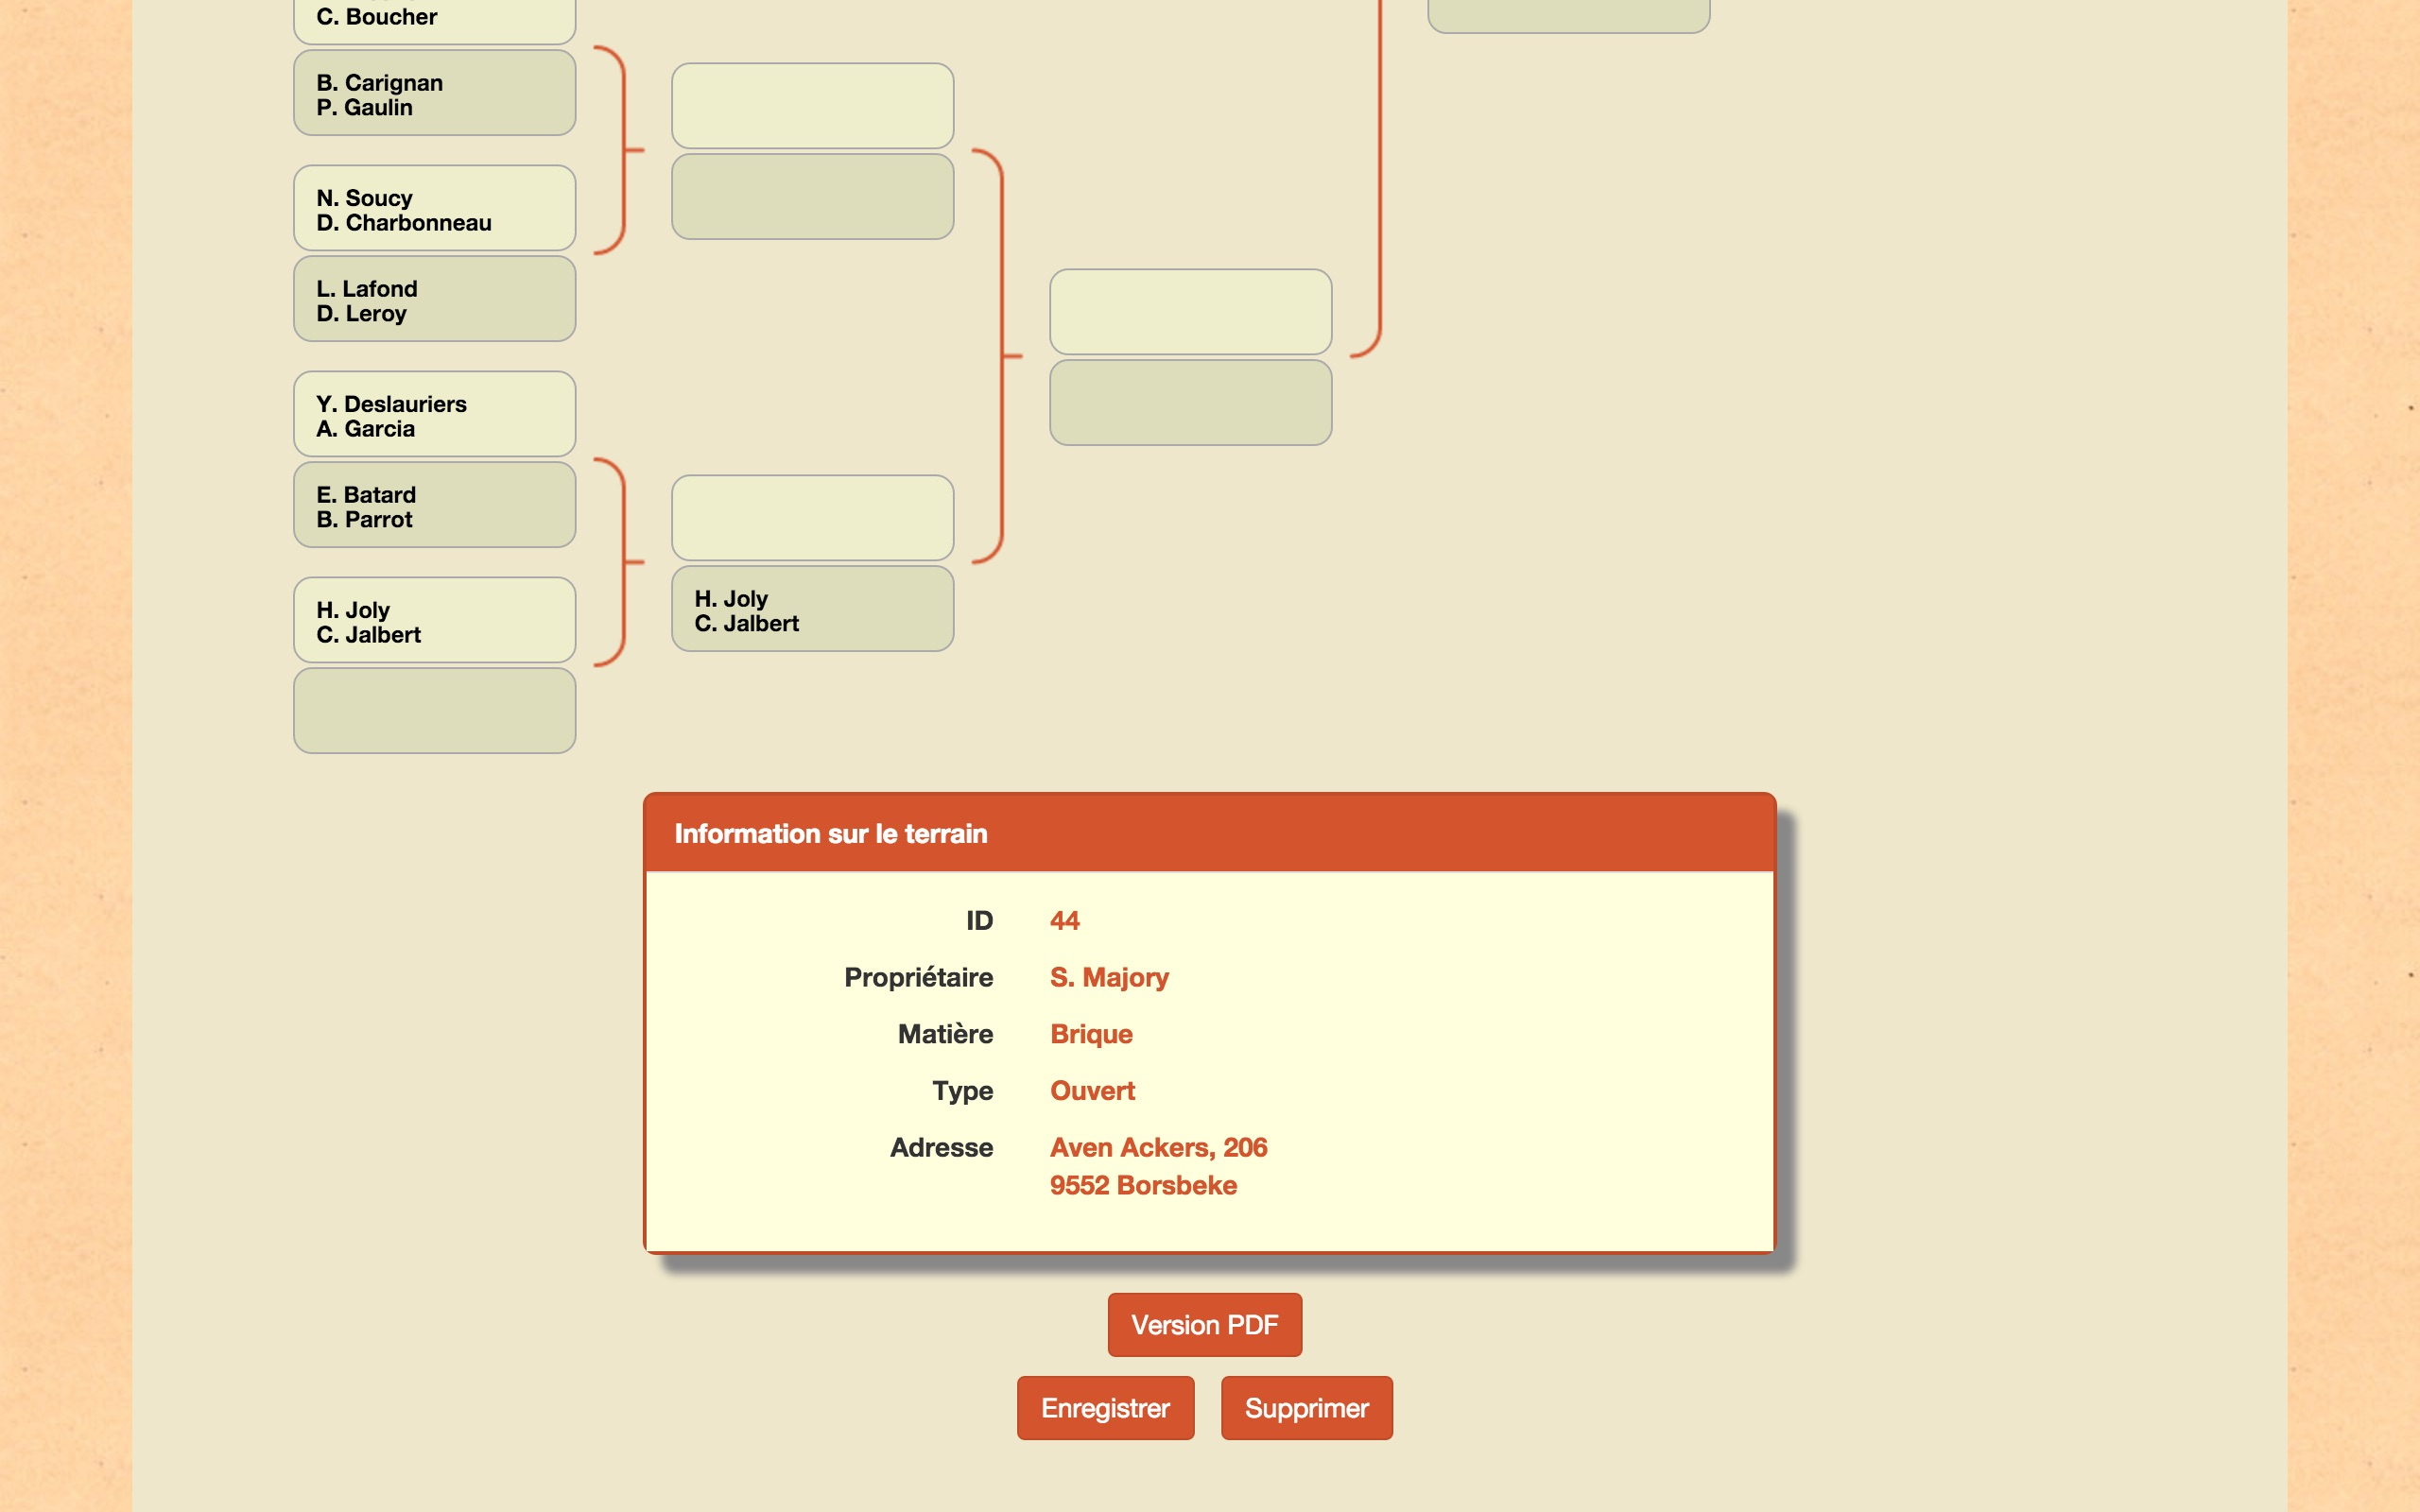
\includegraphics[scale=0.15]{user_images/staff/GererTournois/GererKnockoff/CreerKnockoff/011.jpg}
\caption{Créer une table d'élimination, étape 11}
\end{figure}

\subsection{Supprimer une table d'élimination}

Pour supprimer l'arbre d'élimination d'un tournoi, il faut accéder à la page de l'arbre du tournoi d'élimination, soit en cliquant sur le bouton "Arbre du tournoi" sur la page principale des tournois.\newline

En bas de la page de l'arbre d'élimination, cliquer sur le bouton "Supprimer" pour supprimer l'arbre d'élimination du tournoi.

\begin{figure}[H]
\centering
\includegraphics[scale=0.15]{user_images/staff/GererTournois/GererKnockoff/SupprimerKnockoff/001.jpg}
\caption{Supprimer une table d'élimination, étape 1}
\end{figure}

\begin{figure}[H]
\centering
\includegraphics[scale=0.15]{user_images/staff/GererTournois/GererKnockoff/SupprimerKnockoff/002.jpg}
\caption{Supprimer une table d'élimination, étape 2}
\end{figure}

\begin{figure}[H]
\centering
\includegraphics[scale=0.15]{user_images/staff/GererTournois/GererKnockoff/SupprimerKnockoff/003.jpg}
\caption{Supprimer une table d'élimination, étape 3}
\end{figure}

\subsection{Encoder les scores de la table d'élimination}

Pour encoder les scores de l'arbre du tournoi d'élimination, il suffit d'accéder à la page de l'arbre d'élimination, et de cliquer sur une des paires d'un affrontement.

\begin{figure}[H]
\centering
\includegraphics[scale=0.15]{user_images/staff/GererTournois/GererKnockoff/EncoderKnockoff/001.jpg}
\caption{Encoder les scores d'une table d'élimination, étape 1}
\end{figure}

\begin{figure}[H]
\centering
\includegraphics[scale=0.15]{user_images/staff/GererTournois/GererKnockoff/EncoderKnockoff/002.jpg}
\caption{Encoder les scores d'une table d'élimination, étape 2}
\end{figure}

Une boîte de dialogue propose d'entrer le score du match.

\begin{figure}[H]
\centering
\includegraphics[scale=0.15]{user_images/staff/GererTournois/GererKnockoff/EncoderKnockoff/003.jpg}
\caption{Encoder les scores d'une table d'élimination, étape 3}
\end{figure}

\begin{figure}[H]
\centering
\includegraphics[scale=0.15]{user_images/staff/GererTournois/GererKnockoff/EncoderKnockoff/004.jpg}
\caption{Encoder les scores d'une table d'élimination, étape 4}
\end{figure}

Le gagnant est automatiquement placé à l'étape suivante de l'arbre.

\begin{figure}[H]
\centering
\includegraphics[scale=0.15]{user_images/staff/GererTournois/GererKnockoff/EncoderKnockoff/005.jpg}
\caption{Encoder les scores d'une table d'élimination, étape 5}
\end{figure}

\begin{figure}[H]
\centering
\includegraphics[scale=0.15]{user_images/staff/GererTournois/GererKnockoff/EncoderKnockoff/006.jpg}
\caption{Encoder les scores d'une table d'élimination, étape 6}
\end{figure}

\begin{figure}[H]
\centering
\includegraphics[scale=0.15]{user_images/staff/GererTournois/GererKnockoff/EncoderKnockoff/007.jpg}
\caption{Encoder les scores d'une table d'élimination, étape 7}
\end{figure}
